%
% File:     chapter-systemmodel.tex
% Author:   awl8049
% Revision: $Revision: 1.7 $
%
\chapter{System Modeling}
\label{chp:modelstruct}
In order to develop an energy consumption model based on computational
load of the system, we consider $E_{dc}$, the total DC power input to
the system, at the output of the power supply.  Most servers operate on
the AC input, with efficiency of power conversion from AC to DC equal to
72 - 80 \% (depending on the system load~\cite{ton2008}) and with the DC
output delivered in the domains of +/-12V, +/-5V, and +/-3.3V
\cite{SSI2004}.  Typically, two 12 Vdc lines supply power to the
processor's hard drive(s) and cooling fans in the system.  The 5 Vdc and
3.3 Vdc lines are dedicated to supplying power to the support chips and
peripherals on the board.

Energy delivered to a server system, $E_{dc} = E_{system}$, can be
expressed as a sum of energy consumed by constituent sub-systems in the
server.  Generally, there are five sources of energy consumption in a
server system:
\begin{description}
\item{$E_{proc}$:} Energy consumed in the processor due to computation,
\item{$E_{mem}$:} Energy consumed by DRAM chips,
\item{$E_{hdd}$:} Energy consumed by the hard disk drive(s),
\item{$E_{board}$:} Energy consumed by peripherals in support of board the
  operations, including all devices in multiple voltage domains across the board
  (like chip-set chips, voltage regulators, bus control chips, connectors, interface devices, etc.),
\item{$E_{em}$:} Energy consumed by all electrical and electromechanical
  components in the server, including fans and other support components.
\end{description}

Total energy consumed by the system with a given computational workload
can be expressed as:
\begin{equation}
\label{eq:linmodel}
E_{system}= E_{proc} + E_{mem} + E_{hdd}+ E_{board} +  E_{em}.
\end{equation}
Each of the above terms is explored in turn by following an energy
conservation principle.  In order to get a true measure of the
computational load on the system, our approach snoops on bus
transactions per unit time (indicated by PeC readings), measures the
temperature changes (in die and ambient sensor readings), and records
the speeds of cooling fans, in the course of job execution.  The use of
those PeCs and metric readings fits well to NUMA-based multi-core
processors.
\begin{figure*}[tp]
  \begin{minipage}{0.5\linewidth}
  \centering
     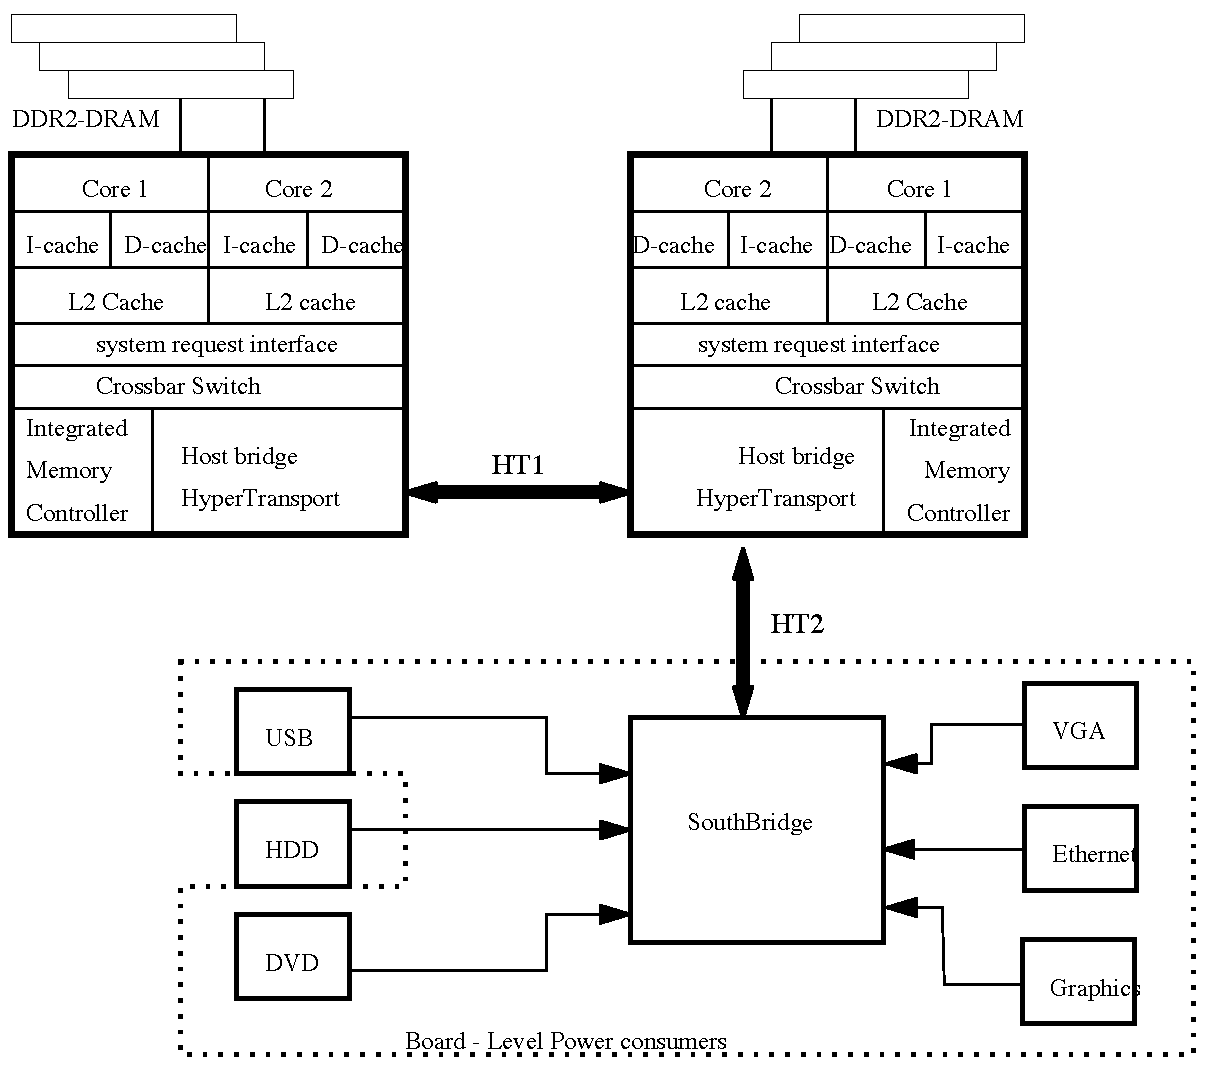
\includegraphics[scale=0.3]{x2200sys}
     \caption{AMD Opteron architecture.}
     \label{fig:amdarch}
  \end{minipage}\hspace{0.1cm}
  \begin{minipage}{0.5\linewidth}
  \centering
     \includegraphics[scale=0.5]{intelnehalem}
     \caption{Intel Xeon (Nehalem) architecture.}
     \label{fig:intarch}
  \end{minipage}
\end{figure*}
\section{Processor energy consumption}
\label{sec:procmodel}
Consider the AMD Operton architecture and the Intel Nehalem
architecture, as depicted in \figurenames~\ref{fig:amdarch} and
\ref{fig:intarch}.  The former is a NUMA-based processor
(\figurename~\ref{fig:amdarch}), with Northbridge functionality
incorporated in the processor core and each core responsible for local
access to the memory connected to that Northbridge logic (shown in
\figurename~\ref{fig:amdarch} as ``Integrated Memory Controller'').
Processor cores on a single die are connected via a crossbar to the
HyperTransport bus (i.e., HT1) between processors.  A coherent bus
protocol is used to ensure memory consistency between processor cores on
each die.  In addition, the master processor in the system is connected
via a second HyperTransport bus (i.e., HT2) to the Southbridge device
that manages connections to the outside world.  A similar structure
exists in the Intel Xeon Nehalem architecture.  Unlike the AMD Operton,
each Nehalem processor is connected to an Input-Output handler, which
provides the Southbridge with connecting functions for off-chip resources.

It is observed that work done by any of the processors, as the heart of
energy consumption in a server system, can be quantified in terms of bus
transactions in and out of the processors.  Traffic on the external
buses provides a measure of how much data is processed by the processor.
Our energy consumption model aims to treat each processor as a black
box, whose energy consumption is a function of its work load (as
manifested by core die temperatures measured at the system level by
\texttt{ipmitool} through sensors on the path of the outgoing airflow
from the processor).  In practice, when estimating processor power
consumption based on PeCs (performance counters), there are only a
limited number of PeCs for tools, like \texttt{cpustat}, to track simultaneously.

For the AMD dual-core Operton architecture (shown in
\figurename~\ref{fig:amdarch}), traffic on the HT buses is viewed as a
representative of the processor workload, reflecting the amount of data
being processed by a processor (i.e., its involved cores).  The HT2 bus
is non-coherent and connects one of the two processors to the
Southbridge (whereas the Northbridge is included on the Opteron
processor die).  Thus, traffic on the HT2 bus reveals hard-disk and
network transactions.  This model scales by considering the effect of
network traffic and disk I/O transactions.  HT1 is a coherent bus
between the two SMP processors and, as such, PeCs on HT1 provide
accurate estimation on the processing load of cores executing jobs.
Per-core die temperature readings are directly affected by the number of
transactions over the HT1 bus.  A similar observation holds for the QPL
links present in the Intel Nehalem architecture, with traffic between
its two cores reflected by transactions on QuickPath Links between the
cores, denoted by $QPL_C$ (see \figurename~\ref{fig:intarch}).

Therefore, total processor power consumption at time $t$, $P_{proc}(t)$,
is related to processor temperature readings and the estimated amount of
data being processed at the time, and it can be expressed as a function
of three metrics: die temperature readings for processors 0 and 1, and
the number of bus transactions (i.e., traffic over HT1 for the AMD
server and over $QPL_C$ for the Intel server).  We have processor energy
consumption between times $t_{1}$ and $t_{2}$ as follows:
\begin{equation}
  \label{eq:procpwr2}
  E_{proc}=\displaystyle\int_{t_{1}}^{t_{2}}\left( {P_{proc}(t)} \right)dt.
\end{equation}
\section{DRAM energy consumption}
\label{sec:dram}
Energy consumed by the DRAM banks is directly related to the number of
DRAM read/write operations involved during the time interval of
interest, and the number is reflected by (1) the last-level cache misses
for all $N$ constituent cores ($CM_{i}(t)$, $i$ = 1, 2, ..., $N$) in
the server when executing jobs and (2) the data amount due to disk
accesses for OS support (like page tables, checkpoints, virtual
environments) and due to performance improvement for peripheral devices
(like buffered data for disks and optical devices, spooled printer
pages).  The data amount in (2) above, named $DB(t)$, is reflected by
traffic over $HT_{2}$ (or QuickPath links between the two cores and the
Input/Output handler, denoted by $QPL_{IO}$) for the AMD Opteron server
(or the Intel Xeon server), as demonstrated in
\figurename~\ref{fig:amdarch} (or \figurename~\ref{fig:intarch}).
This is because network traffic does not exist in either testing server,
which comprises only a single chip.  Additional energy contributors
include activation power and DRAM background power (due to leaking
currents), represented by $P_{ab}$.  As stated earlier
\cite{Micron2007}, DRAM activation power and background power can be
obtained from the DRAM documentation, and they together amount to 493 mW
for one DRAM module in our AMD Opteron server.  Consumed energy over the
time interval between $t_{1}$ and $t_{2}$ can be expressed by
\begin{equation*}
  \label{eq:dram}
  E_{mem}=\displaystyle\int_{t_{1}}^{t_{2}}\left( (\sum_{i=1}^{N}CM_{i}(t)+DB(t))\times
    P_{DR}+P_{ab}\right)dt,
\end{equation*} 
where $P_{DR}$ refers to DRAM read/write power per unit data.
\begin{table}[tp]
\caption{Hitachi HDT725025VLA360 disk power parameters}
\centering
\begin{tabular}{ l l }
\hline
\textbf{Parameter} & \textbf{Value} \\
\hline
  Interface & Serial ATA\\
  Capacity & 250 GB\\
  Rotational speed & 7200 rpm  \\
  Power & \\
  ~~Spin up& 5.25 W (max)\\
  ~~Random read, write & 9.4 W (typical)\\
  ~~Silent read, write & 7 W (typical)\\
  ~~Idle & 5 W (typical)  \\
  ~~Low RPM idle & 2.3 W (typical for 4500 RPM)\\
  ~~Standby & 0.8 W (typical)\\
  ~~Sleep & 0.6 W (typical)\\
\hline
\end{tabular}
\label{tab:hddparam}
\end{table}
\section{Hard disk energy consumption}
\label{sec:networkengery}
Energy consumed by the hard disk(s) is approximated by using a
combination of relevant PeCs and drive ratings.  Both our test servers
use the Hitachi's SATA hard disk (whose specification and relevant power
consumption figures are listed in Table ~\ref{tab:hddparam}).  Based on
the physical, electrical, and electromechanical parameters of a hard
disk, one can construct its detailed power consumption model.  However,
a cruder but simpler model can be obtained from the typical power
consumption data of hard disks and pertinent PeCs, including (1) the
number of reads and writes per second to the disk and (2) the amount of
data (in kilobytes) read from and written to the disk.  Those PeCs can
be measured by the tool of \texttt{iostat}, arriving at approximate disk
power consumption, $E_{hdd}$, as:
\begin{align*}
\label{eq:hddpwr1}
E_{hdd} = &P_{spin-up}\times T_{su}+  P_{read}\sum N_r\times T_r \nonumber\\
        &+ P_{write}\sum N_w\times T_w+ \sum P_{idle}\times T_{id}
\end{align*}
where $P_{spin-up}$ is the power required to spin-up the disk from 0 to
full rotation, and $T_{su}$ is the time required to achieve spin up,
typically about 10 sec.  $P_{read}$ (or $P_{write}$) is the power
consumed per kilobyte of data read from (or written to) the disk,
whereas $N_r$ (or $N_w$) is the number of kilobytes of data reads (or
data writes) in time-slice $T_r$ from (or to) the disk.  The Hitachi
disk achieves read operations at 1.5 Gbits/s, when consuming 530 mA
current at +5V, thereby exhibiting approximately $13.3 \mu W$/Kbyte.
Similarly, it is found to consume $6.67 \mu W$/Kbyte for write
operations.  The numbers of $N_r$ and $N_w$ can be obtained using
\texttt{iostat} according to the chosen time slice.

There are two idle states for the disk: idle and unloaded idle (when
disk read/write heads are unloaded).  The time to go from the unloaded
idle state to the idle state is usually less than 1 second (smaller than
the resolution of \texttt{iostat}).  Thus, a history match count in the
\texttt{iostat} statistics with zero reads and writes signifies the
periods in which the disk is idle, permitting us to compute idle energy
consumption accordingly.  \texttt{iostat} readings for the durations of
switching to different disk power states may be obtained with a more
in-depth analysis, which is not consider in this work.
\section{Board energy consumption}
\label{sec:board}
The quantity of $E_{board}$ represents energy consumption caused by the
support chipsets, control logic, buses, signal links, etc.,
and it usually falls into the 3.3V and 5V power domains.
In our case, this value is obtained using current probe-based measurements.
The results measured over an interval of interest, $t_{interval}$,
excluded the effects of processor, disks, fans, and optical devices, leading to:
\begin{equation}
\label{eq:board}
E_{board} = \left(\sum V_{power-line}\times I_{power-line}\right) \times t_{interval}.
\end{equation}
Note that introducing the current sensors (possibly taking up to 28 for
a server ~\cite{SSI2004}) to the power lines on the board will provide
instantaneous current readings for use in \equationname~(\ref{eq:board}).

Aggregated power consumption effects on the board may be captured using
ambient temperature readings on the board.  Such readings can be
obtained using system management tools commonly found in server
environments (such as IPMI), and they are included in the set of our PeCs
for energy consumption estimation.
\section{Electromechanical energy consumption}
\label{sec:electrical}
A server always involves electromechanical energy consumption, $E_{em}$,
which is mainly due to the electromechanical functions related to system
cooling.  Multiple fans often exist in a server for cooling.  Power
drawn by the $i^{th}$ fan at time $t$ can be given by the following
equation:
\begin{equation}
\label{eq:fanp}
P_{fan}^{i}(t) = P_{base} \times \left(\frac{RPM_{fan}^{i}(t)}{RPM_{base}}\right)^3
\end{equation} 
where $P_{base}$ defines the base power consumption of the unloaded system
when running only the base operating system and no application workload.
The $P_{base}$ value is obtained experimentally by measuring the current drawn
on the +12V and +5V lines, using a current probe and an oscilloscope.
There is a current surge at system start, which is neglected.
Under nominal conditions, the +12V line draws approximately 2.2A
to power both blower fans in the AMD testing server.

A server with $N$ cooling fans results in electromechanical power at time $t$ as
\begin{equation*}
\label{eq:electp}
P_{elect}(t) =  V(t) \cdot I(t) + \sum_{i=1}^NP_{fan}^{i}(t)
\end{equation*} 
where the first term is instantaneous DC power output from the power supply,
representing DC power consumed by the server, and
$P_{fan}^{i}(t)$ is expressed in \equationname~(\ref{eq:fanp}).

Total electromechanical energy consumption over a given task execution
period of $T_{p}$ equals:
\begin{equation*}
\label{eq:elect}
E_{em} =  \int^{T_{p}}_0 \left(V(t) \cdot I(t) + \sum_{i=1}^NP_{fan}^{i}(t)\right)dt.
\end{equation*} 
\begin{figure}[tp]
\begin{center}
     \includegraphics[scale=0.60]{acdcpower2.pdf}
     %\includegraphics[]{acdcpower2.pdf}
     \caption{Proposed power distribution for servers.}
     \label{fig:psu}
\end{center}
\end{figure}
\section{Proposed power distribution}
\label{sec:powerdist}
The input to our derived energy consumption model is current readings at
the power supply lines to the server components.  While not available
yet, current sensors (like MAXIM's 4473~\cite{maxim2006}) may be placed
at the outputs of the power supply unit (PSU, see
\figurename~\ref{fig:psu}) to dynamically track DC power draws during
job execution as system load varies.  A power distribution diagram, with
current sensors incorporated as measurable PeCs, is depicted in
\figurename~\ref{fig:psu}, where a rack-level DC power source is used
for power savings due to its better power efficiency.

With current sensors provided at the output of the DC voltage lines
delivering power to the hard disk drives, for example, one may measure
hard disk power consumption in real-time.  Let the current sensors at
+5V (or +12V) lines to the hard disk be denoted by $v_1(t)$ and $i_1(t)$
or ($v_2(t)$ and $i_2(t)$), which is no larger than 730mA (or 630mA),
we have $E_{hdd}$ as follows:
\begin{equation*}
\label{eq:hddpwr2}
E_{hdd} =  \int_{t1}^{t2} \left( v_1(t)\times i_1(t) + v_2(t)\times i_2(t) \right) dt.
\end{equation*}
Given no current sensors available in our experimental servers, we
obtained the readings by a current probe, logged through an
oscilloscope.

Typically, a server at the idling state (when running the operating
system and no application jobs) consumes some 40 to 42\% of its rated
power (which is 450W in our case).  Conversion efficiency increases to
about 80\% when the server is heavily loaded, and the SMPS regulates the
power supply to work at 75\% conversion efficiency when power drawing is
over 50\% of the rated one.  Hence, conversion losses of the power
supplied to the system is at least 20\%, even for the best conversion
scenario.  Earlier studies \cite{ton2008} have shown that most DC
systems perform better in terms of power efficiency than their AC
counterparts.  A typical AC-based server system has a power supply
efficiency of 73\%, as compared with a 92\% for a DC system.  Also, the
overall system efficiency for an AC system is 61\%, in comparison to
85\% for a DC system.

While a rack level DC power distribution system easily translates into
large power savings at the server level, our model considers a part of
this power conversion unit, since it is not software tunable in its
present state. Currently, our model externally monitors the input power
to the system and controls the power, and consequently, thermal envelope
of the system, based on the processing load.

To understand how our analytical model can be improved by the addition
of such sensors (as valuable PeCs), consider how one might partition
$E_{dc}$ by having access to this information.  Most power supplies
limit the total power delivered through the 5V and 3.3V lines to about
20\% of the rated power supply ($P_R$).  Assuming that each of the
voltage lines in domain $j$, $v_{k}^{j}(t)$, draws current
$i_{k}^{j}(t)$, then each line draws instantaneous power of
$p_{k}^{j}(t) = v_{k}^{j}(t)\cdot i_{k}^{j}(t)$.  Given a voltage domain
with $M_{j}$ DC lines as output, the total power delivered for voltage
domain $j$ is:
\begin{equation*}
\label{eq:power_vdomain}
p_{v}^{j}(t)=  \sum_{k=1}^{M_{j}} v_{k}^{j}(t)\cdot i_{k}^{j}(t)
\end{equation*}

If the board has $N$ voltage domains: $v_{1}$, $v_{2}$, $\ldots$, $v_{N}$,
total DC power delivered into the system equals:
\begin{align*}
\label{eq:power_vtot}
p_{dc}(t) = \sum_{j=1}^{N} p_{v}^{j}(t)\\
         =  \sum_{j=1}^{N} \sum_{k=1}^{M_{j}} v_{k}^{j}(t)\cdot i_{k}^{j}(t).
\end{align*}
Total energy delivered to the system between times $t_2$ and $t_1$ is:
\begin{equation*}
\label{eq:power_input}
E_{dc} = \int_{t_1}^{t_2} p_{dc}(t) dt  = \int_{t_1}^{t_2} \sum_{j=1}^{N} \sum_{k=1}^{Mj} v_{k}^{j}(t)\cdot i_{k}^{j}(t) dt.
\end{equation*}
\clearpage
For the 3.3V and 5V lines, we have the following constraint:
\begin{align*}
\label{eq:power_constr}
E_{dclv} &= \int_{t_1}^{t_2} p_{dclv} (t) dt \nonumber\\
        &=  \int_{t_1}^{t_2} \left( \sum_{k=1}^{M_{1}} v_{k}^{1}(t)\cdot i_{k}^{1}(t) +
        \sum_{k=1}^{M_{2}} v_{k}^{2}(t)\cdot i_{k}^{2}(t) \right) dt \nonumber\\
        & \leq 0.2 P_R
\end{align*}
where $M_{1}$ and $M_{2}$ are the total 3.3V and 5V lines, respectively.
Thus, in our 450W rated system, the power delivered by the 3.3V and 5V lines is capped at 90W.

\section{Thermal  Extensions to the Model}
\label{sec:themalmodel}
There are two metrics of interest for the thermal workload of a
multi-core processor. An application $A$ has a length $L(A,D_{A},t)$
which is the total time of execution $t$ of
the application working upon a set of data $D_{A}$. The
application $A$ is composed of $p$ processes, with each process
associated with a data set of size $d_i$, for $1\leq i \leq p$, in a
single logical CPU. The total data associated with an application $A$ is
the sum of the data associated with its component processes:
\begin{equation}
\label{eq:totaldata}
D_{A}=\displaystyle\sum_{i=1}^p{d_i}.
\end{equation}
We assume that the activities are taking place in a staging area which
contains the main and virtual memory operating spaces, as well as the
processor with its cores and their associated caches and shared cache.
This time of execution measurement includes both computation time and
the time to move the data for the problem from the staging area
(peripherals off the chip like DRAM and HDD) to a computation or
operation area (on the chip such as the caches and the cores).

The second metric of interest is the energy consumption or energy
workload of an application, $U(A,D_{A},t)$. For each application $A$ and
problem size $D_{A}$, we define the the workload $W(p_{i},d_{i},t)$, $1
\leq i \leq p$, in a data-operation dependent and system-independent
way. The workload $W$ contains two components: (1) the operations
count that is performed by the computational core, and (2) the
communication operations required for transfer of data, instructions, and data
coherency and book-keeping operations. These are measured in terms of
the number of bytes operated upon, or number of bytes transferred. Thus
the energy workload of an application $A$ operating on a data set $D_A$
can be expressed as:
\begin{equation}
\label{eq:eworkload}
U(A,D_{A},t) = \displaystyle \lim_{n \to k_e }n \times W(p_i,d_i,t)
\times L_n(A_{n},D_{A_{n}},t), 1\leq i \leq p
\end{equation}
where $L_n(A_{n},D_{A_{n}},t)$ is the total time to execute $n$ applications using
the chip. The term $k_{e}$ is the total number of applications that can be
executed with the associated length of time for $L_n$, at which point a
``thermal event'' will occur causing the applications and the system to
catastrophically fail, or shut down.

It is easy to see that the above term is energy consumption of the
system till a thermal event occurs. In order to relate the energy
expenditure of the system while running applications, to the
corresponding joule heating, we define the term ``Thermal Equivalent of
Application\index{idx:tea}'' (TEA), which is defined as the electrical work converted
to heat in running an application and is measured in terms of die
temperature change and ambient temperature change of the system. Thus for
the application $A$ we express TEA as :
\begin{equation}
\label{eq:tea}
\Theta_A(A,D_{A}, T,t) = \frac{U(A,D_{A},t)}{\displaystyle \lim_{T \to T_{th}} J_e \times (T - T_{nominal})}
\end{equation}
The quantity $T_{th}$ refers to the threshold temperature at which a DTM
triggered event will occur.  $T_{nominal}$ refers to the nominal
temperature as reported by the DTM counters/registers when the system is
in a quiescent state, i.e., only the operating system is running and no
application is being executed. The term $J_{e}$ is the ``electrical
equivalent of heat'' for the chip, which reflects the
\textit{informational entropy}\index{ientropy} of the system associated with processing
the data bits that application $A$ computes and communicates, as well as
the black body thermal properties of the chip packaging and the cooling
mechanisms around the chip. Thus, TEA is a dimensionless quantity with
both denominator and numerator expressing work done or energy consumed
in finishing a task.

For managing the thermal envelope of applications on server systems as
well as embedded systems, we are interested in the thermal efficiency of
the operation, that is, the thermal cost of taking an application to
completion. The thermal efficiency is defined as:
\begin{equation}
\label{eq:thermeff}
\eta(A, D_{A},T,t) = \frac{\Theta_A(A,D_{A}, T,t)}{\Theta_A(A_e,D_{A_{e}}, T_{me}, L_{e})}
\end{equation}
where $T_{me}$ is the maximum temperature which the core will carry
over until a DTM triggered event occurs and $A_e$ refers to the application
whose energy consumption has caused the DTM triggered event to take
place. $L_{e}$ is the execution time of application $A_e$. Thus
$\eta(A, D_{A},T,t)$ is a measure of the ``thermal efficiency of the
application'', which implies how much an application affects temperature
change without compromising it's throughput and/or leads to a thermal
event. Thus the definition of $\eta$ is linked to the definition of the
thermal and energy workload.

We combine these metrics into the achieved performance per unit power
consumed by the chip:
\begin{equation}
\label{eq:thermcost}
C_{\theta}(A, D_{A}, T,t)=\frac{\Theta_A(A,D_{A}, T, t)}{E_{sys}(A,D_{A},t)}
\end{equation}
where $E_{sys}(A,D_{A},t)$ is the overall power consumed during the
application lifetime.  We can apply \equationname~\ref{eq:linmodel} to
\equationname~\ref{eq:thermcost} to apportion the total power consumed
by a single physical component (processor, DRAM units, HDD, motherboard,
and electrical/electromechanical) during the length $L_{A}$ of the
application.

This normalized quantity $C_\theta$ gives some indication of the
``cost'' of executing an application on the given chip.  The problem of
application scheduling requires that we find the best application
ordering that minimizes:
\begin{equation}
\label{eq:thermopt}
  \frac{\partial^{2} C_{\theta}(A, D_{A}, T, t)}{\partial T \partial t}
  =
  \frac{\partial^{2}}{\partial T \partial t}
  \left(
  \Theta_{A}(A,D_{a},T,t)
  \times
  C_{\theta}(A, D_{A}, T,t)
  \right).
\end{equation}

% Following comment block used by GNU-EMACS and AUCTEX packages
% Please do not remove.
%%% Local Variables: 
%%% mode: latex
%%% TeX-master: "prospectus.tex"
%%% End: 
